\documentclass[letterpaper,11pt]{article}
\usepackage[utf8]{inputenc}
\usepackage[margin=1.8cm,left=2.8cm,paper=letterpaper]{geometry}
\usepackage{fullpage}
\usepackage{amssymb}
\usepackage{amsmath}
\usepackage{amsfonts}
\usepackage{bigstrut}
\usepackage{latexsym}
\usepackage{graphicx}
\usepackage{subfigure}
\usepackage{epstopdf}
\usepackage{sectsty}
\usepackage{lipsum}
\usepackage{booktabs}
\usepackage{fancyhdr}
\usepackage{float}
\usepackage{makeidx}
\usepackage[bookmarks = true, colorlinks=true, linkcolor = black, citecolor = black, menucolor = black, urlcolor = black]{hyperref} 
\usepackage[none]{hyphenat}
\usepackage{enumerate}
\usepackage{multicol}
\usepackage[font={small}]{caption}
\usepackage{blindtext}
\usepackage[export]{adjustbox}
\usepackage{listings}
\renewcommand{\tablename}{Tabla}
\renewcommand{\figurename}{Figura}
\renewcommand{\contentsname}
{Índice}



\sectionfont{\centering}

\fancyhf{}
\fancyhead[R]{\textit{ \nouppercase{\rightmark}} }
\fancyfoot[L]{Escuela de Ingeniería y Ciencias}
\fancyfoot[R]{Universidad de Chile}
\fancyfoot[C]{\thepage}
\renewcommand{\headrulewidth}{1pt}
\renewcommand*{\sectionmark}[1]{\markboth{\MakeUppercase{#1}}{}}

\begin{document}
\lstset{language=Java} 

%%%%%%%%%%%%%%%%%%%%%%%%%%Inclusión portada%%%%%%%%%%%%%%%%%%%%%%%%%%%%%%%

	\oddsidemargin 0cm \topmargin -2cm \textheight 21cm \textwidth
	16.5cm \headheight 1cm \linespread {1.0} \headsep 1cm \parindent 0mm

	\begin{titlepage}
  
\includegraphics[width=3cm]{logo.png} 
	\hspace{0cm}
  \begin{tabular}{l}
   \small \scshape{UNIVERSIDAD DE CHILE} \\
 	\small \scshape{FACULTAD DE CIENCIAS FÍSICAS Y MATEMÁTICAS} \\
 	\small \scshape {ESCUELA DE INGENIERÍA Y CIENCIAS} \\
 	\small \scshape{CC3002 - 1 Metodologías de Diseño y Programación} \\
  \vspace*{0.5cm}\mbox{}
  \end{tabular}

\vspace*{3.5 cm}
  
\begin{center}
\fontsize{8mm}{9mm}\selectfont 
	TAREA 2
	
	Resumen

	\vspace*{0.8 cm}
  

\vspace*{3.5 cm}

	% Integrantes
	\normalsize{Daniela Campos} \\
	\normalsize{danielacamposfischer@gmail.com}\\
	\normalsize{https://github.com/DaniCampos/cc3002-tarea2}




	\vspace{0.5 cm}

	% Profesor
	
	\footnotesize{Profesor:} \\
	\vspace{0.08 cm}
	\normalsize{Alexandre Bergel} \\
	
	\vspace{0.5 cm}

	
	% Fechas

	\footnotesize{Fecha:} \\
	\vspace{0.08 cm}
	\normalsize{25 de Octubre del 2017} \\


\end{center}

\end{titlepage}

%\end{document}

	%\topmargin 0cm
	%\pagestyle{empty}
	%\pagestyle{fancy}
	%\pagenumbering{arabic}


%%%%%%%%%%%%%%%%%%%%%%%%%%Comienzo informe%%%%%%%%%%%%%%%%%%%%%%%%%%%



%\newpage

%\begin{center}
%\tableofcontents
%5\end{center}

%\setlength{\parskip}{3mm}



%\section{Diagrama UML}

\center
\section{Diagramas UML}

\begin{figure}[H]
\center
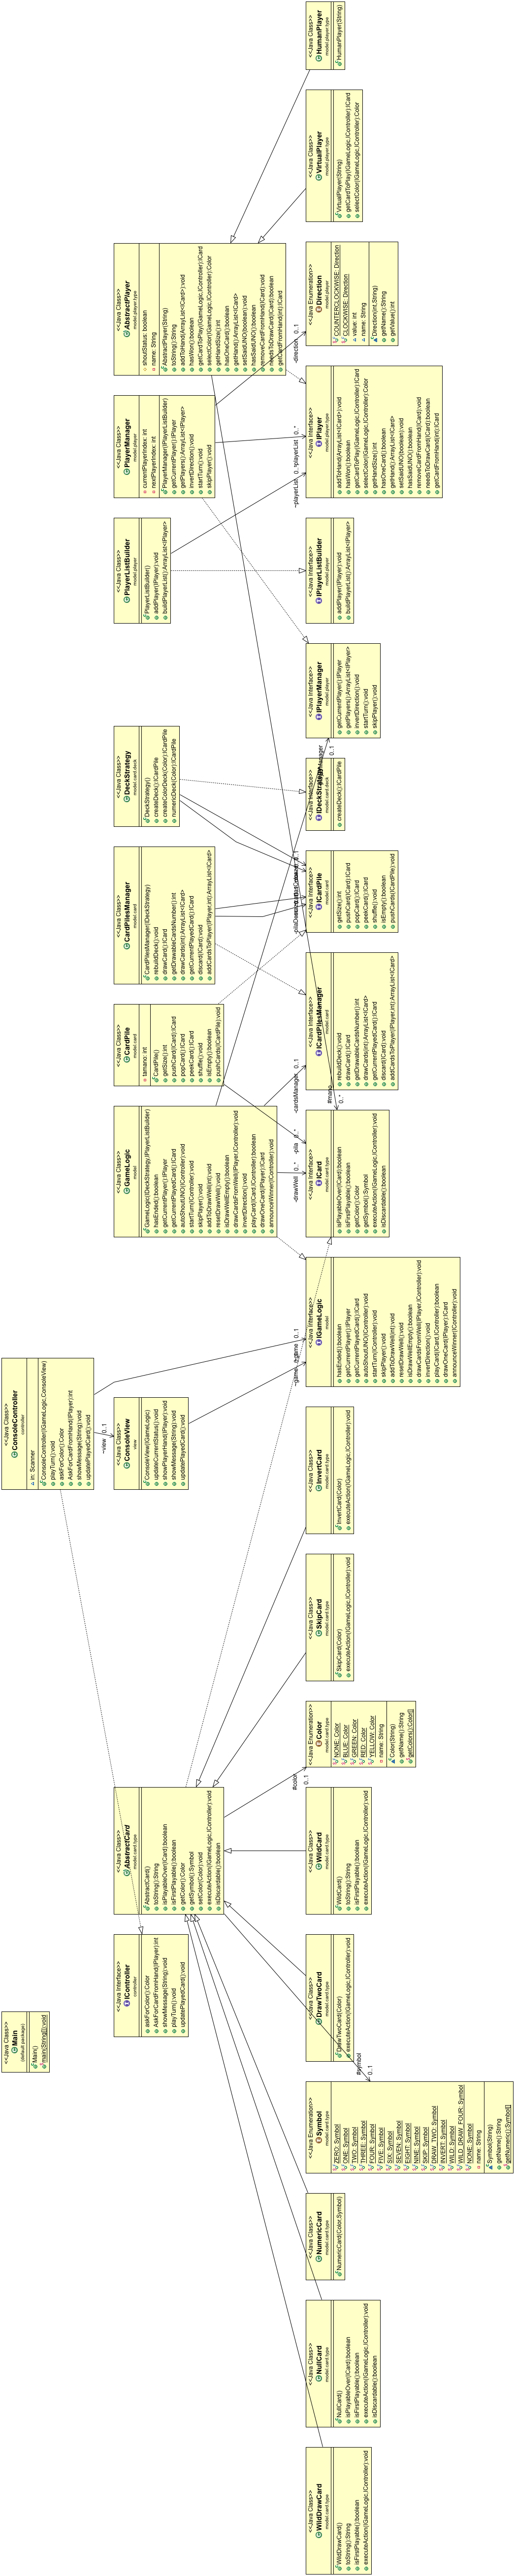
\includegraphics[scale=0.13]{UMLTarea2foto.png}
\caption{UML Proyecto Total}
\end{figure}

\begin{figure}[H]
\center
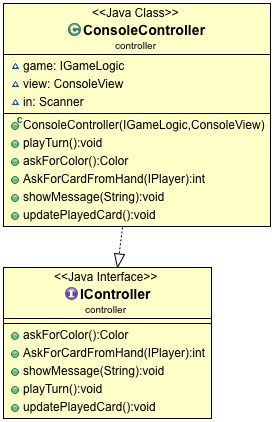
\includegraphics[scale=0.5]{controller.png}
\caption{UML controller.package}
\end{figure}

\begin{figure}[H]
\center
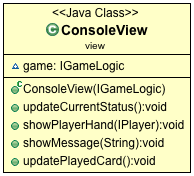
\includegraphics[scale=0.5]{view.png}
\caption{UML view.package}
\end{figure}

\begin{figure}[H]
\center
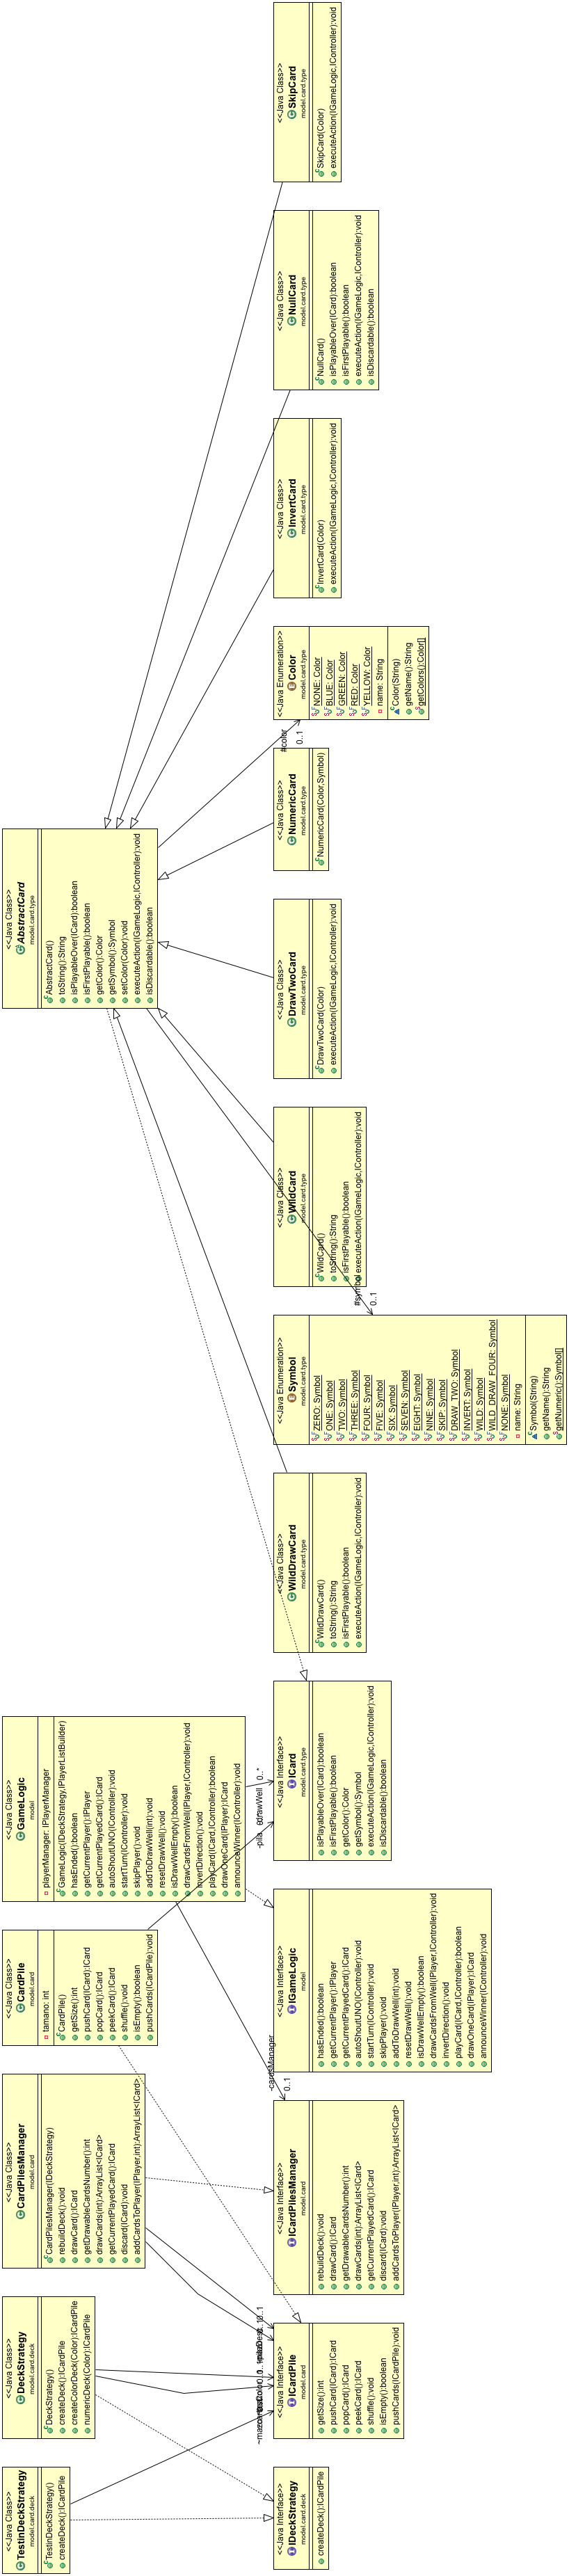
\includegraphics[scale=0.17]{modelCard.png}
\caption{UML modelCard.package}
\end{figure}

\begin{figure}[H]
\center
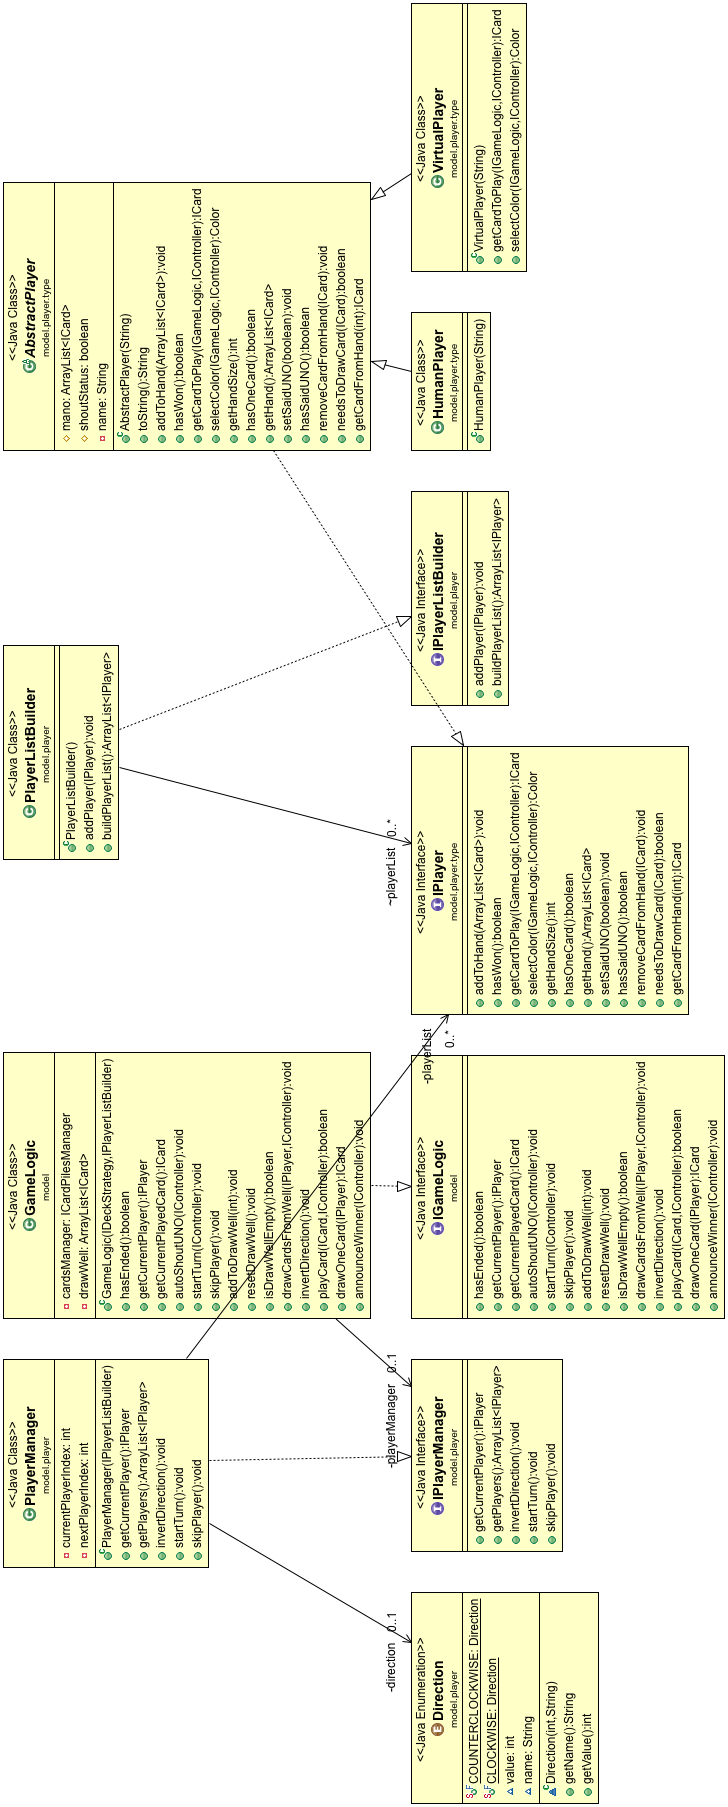
\includegraphics[scale=0.3]{modelPlayer.png}
\caption{UML modelPlayer.package}
\end{figure}
%\begin{figure}
%\centerings
%\includegraphics[scale=0.43]{HeartStone.png}
%\end{figure}

\newpage

\section{Patrones de Diseño}

Los patrones de diseño utilizados en la Tarea 2 fueron:

\begin{enumerate}
\item Adapter: Se adaptó la clase Stack de Java, utlizando la clase ICardPile.

\item Template: Se implementó la clase DeckStrategy, la cual podría ser utilizada para crear un mazo para cualquier juego de cartas, debido a que dentro de esta se implemetaron los métodos createColorDeck y numericDeck, los cuales permiten crear un mazo de cartas de un color y uno con todas las cartas numéricas respectivamente. Se quería implementar una clase TestDeckStrategy, para poder testear la correcta creación de un mazo de cartas, pero por motivos de tiempo no fue posible.

\item NullObject: Se implementó la clase NullCard, con el objetivo de utilizarlo cuando fuera necesario sacar una carta, para así no tener que verificar que el arreglo que contuviera las cartas apropiadas para ser jugadas fuera nulo o estuviera vacío. A la hora de tratar de incorporar este comportamiento al juego, este fallaba, por lo que se priorizó la funcionalidad del juego por sobre la utilización de este patrón.

\item Factory: Se utilizó este patrón a la hora de crear la lista de jugadores y el mazo. Para el caso del mazo, se utilizó la interfaz IDeckStrategy para crear un mazo(Product) utilizando DeckStrategy(Factory), el cliente correspondía a CardPilesManager.  Para crear la lista de jugadores(Producto), se utilizó la interfaz PlayerListBuilder(Factory) utilizando PlayerListBuilder, la cual era instanciada por PlayerManager(Cliente).

\item State: A la hora de realizar este resumen, se pensó en implementar un state patter para distinguir si es que el jugador había dicho uno o no.
\end{enumerate}


\end{document}